% Euclidean Handout Number five
\documentclass{tufte-handout}

%\geometry{showframe}% for debugging purposes -- displays the margins

%%%% Packages to make things pretty
\usepackage{amsmath,amsthm}
\usepackage{booktabs}
\usepackage{graphicx}
\setkeys{Gin}{width=\linewidth,totalheight=\textheight,keepaspectratio}
\graphicspath{{graphics/}}
\usepackage{units}
\usepackage{fancyvrb}
\fvset{fontsize=\normalsize}
\usepackage{multicol}
\usepackage{pdfpages}

%%%% Theorem Evironments
\theoremstyle{definition}
\swapnumbers
\newtheorem{problem}{Problem}[section]
\newtheorem{conjecture}[problem]{Conjecture}
\newtheorem*{definition}{Definition}
\newtheorem*{theorem}{Theorem}
\newtheorem{question}[problem]{Question}
\newtheorem{challenge}[problem]{Challenge}
\newtheorem*{postulate}{Postulate}

%%%%%


\title{Euclidean Geometry:\\An Introduction to Mathematical Work}
\author[]{Math 3600}
\date{Spring 2017} 

\begin{document}

\maketitle
\begin{marginfigure}
    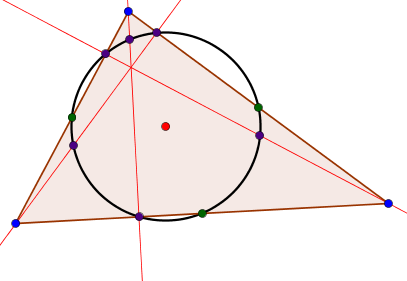
\includegraphics{NPC}
\end{marginfigure}

\setcounter{section}{5}

\section{Polygons}
Now it is time to extend our venue to \emph{polygons} with an arbitrary number of sides.

\begin{definition}\label{defn:n-gon}
Let $n$ be a natural number. An \emph{$n$-gon} is a figure consisting of $n$ points $A_1, A_2, \ldots, A_n$, prescribed in order and called \emph{vertices}, and the $n$ line segments, called \emph{sides}, $A_1A_2, A_2A_3, \ldots, A_{n-1}A_n, A_nA_1$.\\
A \emph{polygon} is an $n$-gon where $n$ has not been specified.
\marginnote[-20pt]{Note: Commonly used terminology includes the following: 3-gon = triangle, 4-gon = quadrilateral, 5-gon = pentagon, 6-gon = hexagon.}
\end{definition}



\begin{problem}\label{prob:exterior-angle}
Suppose that $A,B,C$ are three consecutive vertices of a polygon. 
If at the vertex $B$ we extend one of the two sides through $B$ to a ray, then we create a new angle, called an \emph{exterior angle} to the polygon at $B$.\\
This construction has a choice in it. 
In principle, this could be a problem. 
Describe the problem, then state and prove a theorem that resolves the issue.
\end{problem}




\begin{conjecture}\label{conj:ext-angles-pentagon}
The exterior angles of a pentagon, one choice made at each vertex, add up to four right angles.
\end{conjecture}


\begin{question}\label{question-induction}
What is the sum of the exterior angles of a hexagon? 
What about a general $n$-gon? 
Can you find a way to build on our understanding from small values of $n$, to general values of $n$?
\end{question}



\vfill
\end{document}